\input{../../common/slide-common-header.tex}
\input{../../common/slide-plan.tex}

\title[]{Lecture \basicTwoNum: \basicTwoTopic}
\subtitle[]{\basicTwoKey}
\author[]{Alexander Filatov\\ filatovaur@gmail.com}

\date{}

\begin{document}

\begin{frame}
  \titlepage
    \url{https://github.com/Svazars/parallel-programming/blob/main/slides/pdf/l3.pdf}
\end{frame}

\begin{frame}{In previous episodes}

\begin{itemize} 
 \item Every thread has its own speed and scenario of execution
 \item We expect OS could pre-empt any thread at any time
 \item Interleaving model thread-safety: all operations with data structure 
 \begin{itemize} 
    \item are non-overlapping intervals on single timeline
    \item are consistent with each other in single-threaded sense
 \end{itemize} 
 \item \textbf{Mutual exclusion}: not more than one thread in critical section
 \item \textbf{Deadlock-freedom}: some thread eventually enters critical section
 \item \textbf{Starvation-freedom}: every thread eventually enters critical section
 \item Mutex design space: reentrancy, admission policy, fairness 
 \item Mutex patterns: code locking, data locking, lock splitting
 \item Mutex best practices: recursive locks, encapsulation, leaf locking
 \item Documentation is you best friend
 \end{itemize}
\end{frame}

\begin{frame}{Lecture plan}
\tableofcontents
\end{frame}

\section{Decoupling tasks from threads}
\subsection{Executor}

\begin{frame}[t,fragile]{Useful interfaces}

Runnable\footnote{\tiny\url{https://docs.oracle.com/en/java/javase/11/docs/api/java.base/java/lang/Runnable.html}}
\begin{minted}{java}
interface Runnable {
    void run();
}
\end{minted}

\begin{itemize}
    \item separate task (\textbf{what} to do) from environment (\textbf{where} to do)
\end{itemize}
\end{frame}

\questiontime{\texttt{Runnable.run} should be thread-safe?}

\begin{frame}[t,fragile,noframenumbering]{Useful interfaces}

\begin{minted}{java}
    interface Runnable { void run(); }
\end{minted}
\begin{itemize}
    \item separate task (\textbf{what} to do) from environment (\textbf{where} to do)
\end{itemize}

\pause

ThreadFactory\footnote<2->{\tiny\url{https://docs.oracle.com/en/java/javase/11/docs/api/java.base/java/util/concurrent/ThreadFactory.html}}

\begin{minted}{java}
interface ThreadFactory {
  Thread newThread(Runnable r);
}
\end{minted}

\begin{itemize}
    \item separate environment (\textbf{what} available) from particular thread (\textbf{who} will do)
\end{itemize}
\end{frame}

\questiontime{\texttt{ThreadFactory.newThread} that returns ''previously used'' \texttt{Thread} instance: what are pros and cons?}

\begin{frame}[t,fragile,noframenumbering]{Useful interfaces}

\begin{minted}{java}
    interface Runnable { void run(); }
\end{minted}
\begin{itemize}
    \item separate task (\textbf{what} to do) from environment (\textbf{where} to do)
\end{itemize}

\begin{minted}{java}
    interface ThreadFactory { Thread newThread(Runnable r); }
\end{minted}

\begin{itemize}
    \item separate environment (\textbf{what} available) from particular thread (\textbf{who} will do)
\end{itemize}

\pause

Executor\footnote<2->{\tiny\url{https://docs.oracle.com/en/java/javase/11/docs/api/java.base/java/util/concurrent/Executor.html}}

\begin{minted}{java}
interface Executor {
  void execute(Runnable command);
}
\end{minted}

\begin{itemize}
    \item separate task submission (\textbf{how} distribute work) from the mechanics of how each task will be run (\textbf{who} will do, \textbf{when} will do)
\end{itemize}

\end{frame}

\questiontime{\texttt{Executor.execute} that performs task in the caller thread is OK?}

\begin{frame}[t,fragile]{Using executor}
\begin{minted}{java}
  Executor executor = anExecutor();
  executor.execute(new RunnableTask1());
  executor.execute(new RunnableTask2());
\end{minted}
\end{frame}

\questiontime{Do we need to use locks when using properly implemented thread-safe \texttt{Executor}?}

\begin{frame}[t,fragile]{Using executor}

\begin{minted}{java}
static long total = 0;
static Lock lock = new ReentrantLock();
static long compute(long input) { ... }
static void foo() {
  Executor executor = anExecutor();
  executor.execute( () -> {
        long tmp = compute(1);
        lock.lock(); try { total += tmp; } finally { lock.unlock(); }
  });
  executor.execute( () -> {
        long tmp = compute(2);
        lock.lock(); try { total += tmp; } finally { lock.unlock(); }
  });
\end{minted}
\end{frame}

\begin{frame}[fragile]{ThreadPerTaskExecutor}

\begin{minted}{java}
class ThreadPerTaskExecutor implements Executor {
  private final ThreadFactory factory;
  public ThreadPerTaskExecutor(ThreadFactory f) {
    factory = f;
  }
  public void execute(Runnable r) {
    factory.newThread(r).start();
  }
}
\end{minted}
\end{frame}

\questiontime{\texttt{Executor.execute} declares ''fire-and-forget'' API. Is it enough?}

\subsection{ExecutorService}
\showTOCSub

\begin{frame}[t,fragile]{Even more useful interfaces}

Callable<V>\footnote{\tiny\url{https://docs.oracle.com/en/java/javase/11/docs/api/java.base/java/util/concurrent/Callable.html}}
\begin{minted}{java}
interface Callable<V> {
  V call() throws Exception;
}
\end{minted}

\begin{itemize}
    \item computation has 2 possible outcomes: value \texttt{V} or exception
\end{itemize}
\end{frame}

\questiontime{some thread experienced uncaught exception. Should we \texttt{exit} our program?}

\begin{frame}[t,fragile]{Even more useful interfaces}

\begin{minted}{java}
    interface Callable<V> { V call() throws Exception; }
\end{minted}

\begin{itemize}
    \item computation has 2 possible outcomes: value \texttt{V} or exception
\end{itemize}

\pause

Future<V>\footnote<2->{\tiny\url{https://docs.oracle.com/en/java/javase/11/docs/api/java.base/java/util/concurrent/Future.html}}
\begin{minted}{java}
interface Future<V> {
  V get();
  boolean isDone();
}
\end{minted}

\begin{itemize}
    \item represents the result of an asynchronous computation
\end{itemize}
\end{frame}

\questiontime{what should \texttt{Future.get} return for \texttt{Callable<V>} that failed with exception?}

\begin{frame}[t,fragile,noframenumbering]{Even more useful interfaces}

\begin{minted}{java}
    interface Callable<V> { V call() throws Exception; }
\end{minted}

\begin{itemize}
    \item computation has 2 possible outcomes: value \texttt{V} or exception
\end{itemize}

\begin{minted}{java}
    interface Future<V> { 
        V get();
        boolean isDone(); 
    }
\end{minted}

\begin{itemize}
    \item represents the result of an asynchronous computation
    \item throws \texttt{ExecutionException} if the computation threw an exception
\end{itemize}

\pause

\textbf{Reminder}: \texttt{Thread.join} does not propagate exceptions (see Task 1.1)

\end{frame}


\begin{frame}[fragile]{ExecutorService: beginning}

ExecutorService\footnote{\tiny\url{https://docs.oracle.com/en/java/javase/11/docs/api/java.base/java/util/concurrent/ExecutorService.html}}

\begin{minted}{java}
interface ExecutorService extends Executor {
  void execute(Runnable command);
  <T> Future<T> submit(Callable<T> task);
  <T> List<Future<T>> invokeAll(Collection<? extends Callable<T>> tasks);
}
\end{minted}

\begin{itemize}
    \item features asynchronous computation
    \item allows bulk submission of tasks
\end{itemize}

\end{frame}


\begin{frame}[t,fragile]{Reminder: ThreadPerTaskExecutor}

\begin{minted}{java}
class ThreadPerTaskExecutor implements Executor {
  private final ThreadFactory factory;
  public ThreadPerTaskExecutor(ThreadFactory f) { factory = f; }
  public void execute(Runnable r) { factory.newThread(r).start(); }
}
\end{minted}

\pause
\texttt{ThreadPerTaskExecutor}\textbf{Service}:
\begin{itemize}
    \item features asynchronous computation (\texttt{submit} returns \texttt{Future})
    \item allows bulk submission of tasks (\texttt{submit(Collection)})
\end{itemize}

\end{frame}

\begin{frame}[t,fragile,noframenumbering]{ThreadPerTaskExecutorService}

\begin{minted}{java}
class ThreadPerTaskExecutorService implements ExecutorService {
  private final ThreadFactory factory;
  public ThreadPerTaskExecutorService(ThreadFactory f) { factory = f; }
  public void execute(Runnable r) { 
    ???
  }
  <T> List<Future<T>> invokeAll(Collection<? extends Callable<T>> tasks) {
    ???
    ???
    ???
  }
  <T> Future<T> submit(Callable<T> task) {
    ???
  }}
\end{minted}
\end{frame}


\begin{frame}[t,fragile,noframenumbering]{ThreadPerTaskExecutorService}

\begin{minted}{java}
class ThreadPerTaskExecutorService implements ExecutorService {
  private final ThreadFactory factory;
  public ThreadPerTaskExecutorService(ThreadFactory f) { factory = f; }
  public void execute(Runnable r) { 
    this.submit(() -> { r.run(); return null });
  }  
  <T> List<Future<T>> invokeAll(Collection<? extends Callable<T>> tasks) {
    ???
    ???
    ???
  }
  <T> Future<T> submit(Callable<T> task) {
    ???
  }}
\end{minted}
\end{frame}

\begin{frame}[t,fragile,noframenumbering]{ThreadPerTaskExecutorService}

\begin{minted}{java}
class ThreadPerTaskExecutorService implements ExecutorService {
  private final ThreadFactory factory;
  public ThreadPerTaskExecutorService(ThreadFactory f) { factory = f; }
  public void execute(Runnable r) { 
    this.submit(() -> { r.run(); return null });
  }
  <T> List<Future<T>> invokeAll(Collection<? extends Callable<T>> tasks) {
    var result = new ArrayList<Future<T>>();
    for (var t : tasks) { result.add(this.submit(t)); }
    return result;
  }
  <T> Future<T> submit(Callable<T> task) {
    ???
  }}
\end{minted}
\end{frame}

\begin{frame}[t,fragile]{ThreadPerTaskExecutorService + JoinFuture}

\begin{minted}{java}
class ThreadPerTaskExecutorService implements ExecutorService {    
  <T> Future<T> submit(Callable<T> task) {
    ???
    ???
    ???
    ???
  }
}





\end{minted}
\end{frame}


\begin{frame}[t,fragile,noframenumbering]{ThreadPerTaskExecutorService + JoinFuture}

\begin{minted}{java}
class ThreadPerTaskExecutorService implements ExecutorService {    
  <T> Future<T> submit(Callable<T> task) {
    var future = new JoinFuture();
    future.thread = factory.newThread(() -> { future.result = task.call(); });
    future.thread.start();
    return future;        
  }
}






\end{minted}
\end{frame}

\begin{frame}[t,fragile,noframenumbering]{ThreadPerTaskExecutorService + JoinFuture}

\begin{minted}{java}
class ThreadPerTaskExecutorService implements ExecutorService {    
  <T> Future<T> submit(Callable<T> task) {
    var future = new JoinFuture();
    future.thread = factory.newThread(() -> { future.result = task.call(); });
    future.thread.start();
    return future;        
  }
}
class JoinFuture<V> implements Future<V> {
  Thread thread; 
  V result;
  public V get() { ??? }
  public boolean isDone() { ??? }
}
\end{minted}
\end{frame}


\begin{frame}[t,fragile,noframenumbering]{ThreadPerTaskExecutorService + JoinFuture}

\begin{minted}{java}
class ThreadPerTaskExecutorService implements ExecutorService {    
  <T> Future<T> submit(Callable<T> task) {
    var future = new JoinFuture();
    future.thread = factory.newThread(() -> { future.result = task.call(); });
    future.thread.start();
    return future;        
  }
}
class JoinFuture<V> implements Future<V> {
  Thread thread; 
  V result;
  public V get() { thread.join(); return result; }
  public boolean isDone() { return !thread.isAlive(); }
}
\end{minted}
\end{frame}

\questiontime{there are no locks to guard \texttt{JoinFuture.thread} and \texttt{JoinFuture.result}. Is it OK?}

\begin{frame}[t,fragile]{ThreadPerTaskExecutorService + JoinFuture = Homework}

{\tiny\url{https://github.com/Svazars/parallel-programming/blob/main/hw/block1/3.1/readme.markdown}}
\begin{homeworkmail}{Task 3.1}
    \begin{itemize}
        \item Implement \texttt{ThreadPerTaskExecutorService}
        \item Implement \texttt{JoinFuture} that properly supports exceptions
    \end{itemize}
\end{homeworkmail}
\end{frame}

\questiontime{what are negative sides for starting brand new thread for every submitted task?}

\subsection{Thread pooling}
\showTOCSub

\begin{frame}{Thread pooling}

\begin{itemize}
    \item \texttt{Thread} is valuable and scarce OS resource. 
    \begin{itemize} \item Caching could help. \end{itemize}
    \item Too many \texttt{Thread}s may slow-down each other (oversubscription). 
    \begin{itemize} \item Soft and hard limits could help. \end{itemize}
    \item Most of the computations do not care which thread is used. 
    \begin{itemize} \item Decoupling tasks from carriers could help. \end{itemize}
    \item \texttt{Thread}s may have purpose and context (name, priority, task-specific limits).
    \begin{itemize} \item  Should be properly reflected in observability API. \end{itemize}
\end{itemize}
\end{frame}

\begin{frame}[t,fragile]{SingleThreadExecutor + LockedFuture}

\textbf{Idea:}
\begin{itemize}
    \onslide<4->{\item Lock-per-Future for \texttt{get/set} synchronization}
    \onslide<3->{\item Thread-safe FIFO container for submitted tasks}
    \onslide<2->{\item Only one thread to execute all tasks}
\end{itemize}
\end{frame}


\begin{frame}[t,fragile,noframenumbering]{SingleThreadExecutor + LockedFuture}

\begin{itemize}
    \item Lock-per-Future for \texttt{get/set} synchronization
\end{itemize}

\pause
\begin{minted}{java}
class LockedFuture<V> implements Future<V> {
  final Lock l = new ReentrantLock(); final Callable<V> task;
  V result; boolean done = false;
  public LockedFuture(Callable<V> task) { this.task = task; }
  void setResult(V v) { 
    l.lock(); try { result = v; done = true; } finally { l.unlock(); }}
  V get() {
    while (!isDone()) { /* await task completion */ }
    l.lock(); try { return result; } finally { l.unlock(); }
  }
  boolean isDone() { l.lock(); try { return done; } finally { l.unlock(); }}
}
\end{minted}
\end{frame}


\begin{frame}[t,fragile,noframenumbering]{SingleThreadExecutor + LockedFuture}

\begin{itemize}
    \item Lock-per-Future for \texttt{get/set} synchronization
    \item Thread-safe FIFO container    
\end{itemize}

\pause
\begin{minted}{java}
class LockedFIFO<T> implements Queue<T> {
  private final Queue<T> q = new LinkedList<>();
  private final Lock l = new ReentrantLock();
  boolean offer(T e){ l.lock(); try { return q.offer(e); } finally { l.unlock(); }}
  T poll()          { l.lock(); try { return q.poll();   } finally { l.unlock(); }}
  boolean isEmpty() { l.lock(); try { return q.isEmpty();} finally { l.unlock(); }}
  ...
}
\end{minted}
\end{frame}

\begin{frame}[t,fragile,noframenumbering]{SingleThreadExecutor + LockedFuture}

\begin{itemize}
    \item Lock-per-Future for \texttt{get/set} synchronization
    \item Thread-safe FIFO container for submitted tasks    
\end{itemize}

\pause
\begin{minted}{java}
class SingleThreadExecutor implements ExecutorService {
  private final ThreadFactory factory;
  private final Queue<LockedFuture<?>> queue = new LockedFIFO<>();
  public SingleThreadExecutor(ThreadFactory f) { factory = f; }
  <T> Future<T> submit(Callable<T> task) {
    var future = new LockedFuture<>(task);
    queue.offer(future);
    return future;
  }
}
\end{minted}
\end{frame}

\begin{frame}[t,fragile,noframenumbering]{SingleThreadExecutor + LockedFuture}

\begin{itemize}
    \item Lock-per-Future for \texttt{get/set} synchronization
    \item Thread-safe FIFO container for submitted tasks
    \item Only one thread to execute all tasks    
\end{itemize}

\pause
\begin{minted}{java}
class SingleThreadExecutor implements ExecutorService {
  private final ThreadFactory factory;
  private final Queue<LockedFuture<?>> queue = new LockedFIFO<>();
  private final Thread worker = factory.newThread(() -> {
    while (true) {
      while (queue.isEmpty()) { /* await new task */ }
      var f = queue.poll();
      f.setResult(f.task.call());
    }});
}
\end{minted}
\end{frame}

\questiontime{
\newline
\texttt{LockedFuture.get: while (!isDone()) \{ /* await task completion */ \}}
\newline
\texttt{SingleThreadExecutor: while (queue.isEmpty()) \{ /* await new task */ \}}
\newline
\newline
Could you spot \textbf{performance} problem here?
}

\section{Backoff policies}
\showTOC

\begin{frame}[fragile]{NoBackoff policy}

\begin{minted}{java}
while (true) {
    if (isDone()) {
        break;
    }
    // immediately try again
}
\end{minted}

\begin{itemize}
    \pause \item Pro: highest possible response time. Could be blazingly fast, especially when polling thread does not context switch
    \pause \item Con: could waste CPU time
    \pause \item Con: could cause starvation
\end{itemize}
\end{frame}

\questiontime{What should thread do when task is not yet ready?}

\begin{frame}[fragile]{FixedBackOff policy}

\begin{minted}{java}
while (true) {
    if (isDone()) {
        break;
    }
    Thread.sleep(CONSTANT);
}
\end{minted}

\begin{itemize}
    \pause \item Pro: easy to implement
    \pause \item Pro: predictable
    \pause \item Pro: saves CPU resources
    \pause \item Con: optimal \texttt{CONSTANT} could be task-specific, CPU-specific, workload-specific 
    \begin{itemize}
        \pause \item could cause starvation (too small delay)
        \pause \item could cause latency problems (adds delay to observed pauses)
        \pause \item could cause throughput degradation (too big delay)
    \end{itemize}
\end{itemize}      
\end{frame}

\begin{frame}[fragile]{ExponentialBackOff policy}

\begin{minted}{java}
long current_delay = START_DELAY;
while (true) {
    if (isDone()) {
        break;
    }
    sleep(current_delay);
    current_delay = min(current_delay * 2, MAX_DELAY);
}
\end{minted}

\begin{itemize}
    \pause \item Pro: saves CPU resources
    \pause \item Pro: latency-friendly
    \pause \item Con: still not perfect responsiveness    
\end{itemize}

\pause
We need something better than polling (sleep-and-retry)!
\end{frame}


\section{Signalling}
\showTOC

\begin{frame}[t,fragile,noframenumbering]{Signalling}
\framesubtitle{Motivation}

Thread offloads tasks to other threads and waits for completion.

Polling with backoff: ''time-to-react'' (latency) vs. ''unproductive time'' (throughput).

\pause
We need to
\begin{itemize}
 \item subscribe on completion event
 \item notify subscribers (other threads) in efficient way
\end{itemize}

We need some support from OS!
\end{frame}


\begin{frame}{Signalling}
\framesubtitle{Idea}

Blocking API:
\begin{itemize}
    \item \texttt{wait} (a.k.a. \texttt{await}, \texttt{subscribe} ...)
\end{itemize}

\pause
What are we waiting for?

\begin{itemize}
 \item Some task to be completed (execution flow control)
 \item Some data to be available (data flow control)
\end{itemize}

\pause

Non-blocking API:
\begin{itemize}
    \item \texttt{notify} (\texttt{notify\_one}, \texttt{signal} ...)
    \item \texttt{notifyAll} (\texttt{signalAll}, \texttt{broadcast} ...)
\end{itemize}

\pause
Who is going to be notified?

\pause
\begin{itemize}
    \item Only threads interested in communication
    \item The one/ones that are now suspended in \texttt{wait} method
\end{itemize}

\pause

Must avoid race conditions and data races!
\end{frame}

\questiontime{concurrency primitive that you already know that helps to avoid data races?}

\section{Condition variable}
\subsection{API}
\showTOCSub

\begin{frame}[fragile]{Condition variable API}

Creation\footnote{\tiny\url{https://docs.oracle.com/en/java/javase/11/docs/api/java.base/java/util/concurrent/locks/Lock.html#newCondition()}}:
\begin{minted}{java}
interface Lock {
    Condition newCondition();
}
\end{minted}

Operations\footnote{\tiny\url{https://docs.oracle.com/en/java/javase/11/docs/api/java.base/java/util/concurrent/locks/Condition.html}}:
\begin{minted}{java}
interface Condition {
    void await();
    void signal();
    void signalAll();
}
\end{minted}
\end{frame}

\begin{frame}[fragile]{Condition variable}
\framesubtitle{Usage rules}

Illegal operations:
\begin{itemize}
    \item \texttt{await} out of critical section
    \item \texttt{signal} out of critical section
\end{itemize}

Important details:
\begin{itemize}
    \item \texttt{await} unlocks mutex and starts listening for notification \textbf{atomically}
    \item \texttt{await} wake-ups (consumes notification) and \textbf{starts} mutex acquisition
    \item \texttt{signal/signalAll} wakes up waiting thread(s) only
\end{itemize}
\end{frame}

\begin{frame}{Condition variable}
\framesubtitle{Overview}

\begin{tikzpicture}[remember picture,overlay]
\node[xshift=4cm,yshift=-6.0cm] at (current page.center) {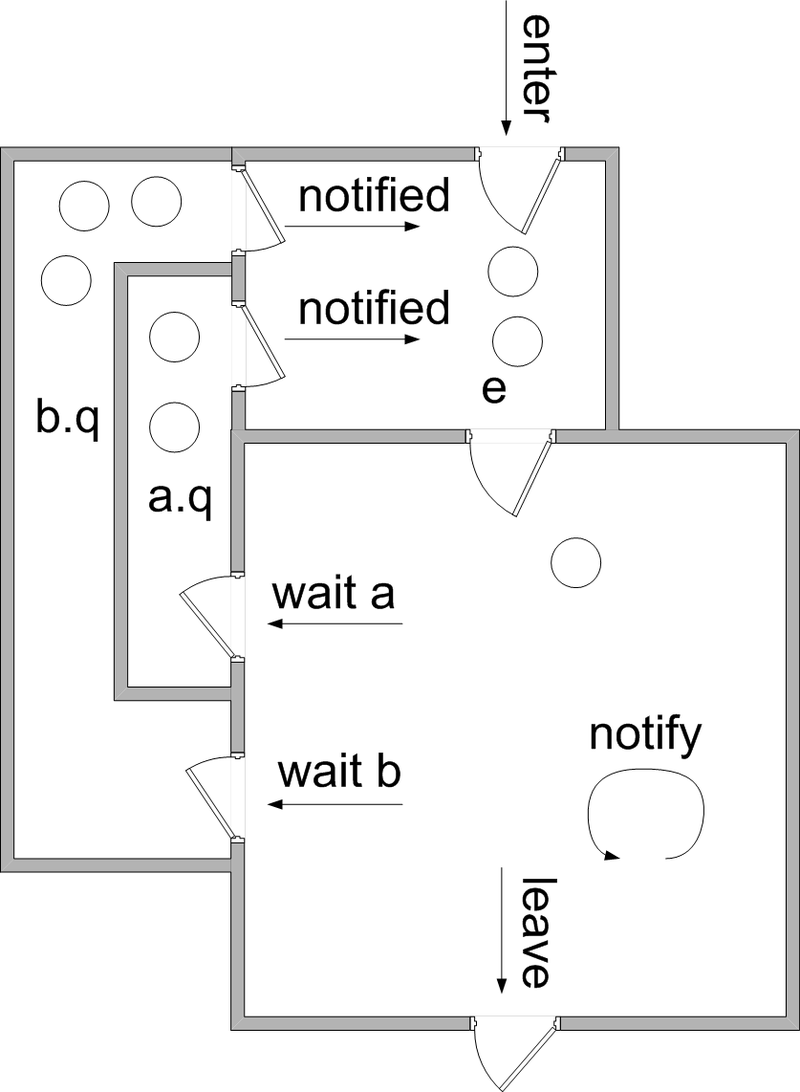
\includegraphics[width=0.35\textwidth]{./pics/CondScheme.png}};
\end{tikzpicture}

One of possible high-level designs\footnote{\tiny\url{https://en.wikipedia.org/wiki/Monitor_(synchronization)#/media/File:Monitor_(synchronization)-Mesa.png}}:
\begin{itemize}
    \pause \item Mutex: Owner
    \begin{itemize}
        \item The only thread inside critical section        
    \end{itemize}
    \pause \item Mutex: EnterSet
    \begin{itemize}
        \item Threads trying to enter critical section
        \item Admission policy for lock acquisition
    \end{itemize}
    \pause \item Condition: WaitSet
    \begin{itemize}
        \item Threads waiting for signal and now out of critical section
        \item Admission policy for notification
    \end{itemize}    
\end{itemize}

\pause
\textbf{Important}: notified threads need to re-enter mutex

% TODO: DaveDice wait morphing pub
\end{frame}


\begin{frame}[t,fragile]{Reminder: LockedFuture}

\begin{minted}{java}
class LockedFuture<V> implements Future<V> {
  final Lock l = new ReentrantLock(); 
  final Callable<V> task;
  V result; 
  boolean done = false;
  public LockedFuture(Callable<V> task) { this.task = task; }
  ...
\end{minted}
\end{frame}

\begin{frame}[t,fragile,noframenumbering]{Reminder: LockedFuture}

\begin{minted}{java}
class LockedFuture<V> implements Future<V> { Lock l; V result; boolean done;  
  void setResult(V v) { 
    l.lock(); try { result = v; done = true; } finally { l.unlock(); }
  }
  V get() {
    while (!isDone()) { /* await task completion */ } // <-----------------
    l.lock(); try { return result; } finally { l.unlock(); }
  }
  boolean isDone() { l.lock(); try { return done; } finally { l.unlock(); }}
}
\end{minted}
\end{frame}

\begin{frame}[t,fragile,noframenumbering]{BetterFuture: using condition variables}

\begin{minted}{java}
class BetterFuture<V> implements Future<V> { Lock l; V result; boolean done;
  final Condition c = l.newCondition();
  V get() { ??? }


  
  void setResult(V v) { ??? }
\end{minted}
\end{frame}


\begin{frame}[t,fragile]{BetterFuture: using condition variables}

\begin{minted}{java}
class BetterFuture<V> implements Future<V> { Lock l; V result; boolean done;
  final Condition c = l.newCondition();
  V get() { l.lock(); try {
              ???
              ???
            } finally { l.unlock(); }}
  void setResult(V v) { 
            l.lock(); try { 
              ???
              ???
            } finally { l.unlock(); }}}
\end{minted}
\end{frame}

\begin{frame}[t,fragile,noframenumbering]{BetterFuture: using condition variables}

\begin{minted}{java}
class BetterFuture<V> implements Future<V> { Lock l; V result; boolean done;
  final Condition c = l.newCondition();
  V get() { l.lock(); try {
              c.await(); 
              return result; 
            } finally { l.unlock(); }}
  void setResult(V v) { 
            l.lock(); try { 
              result = v; done = true;
              c.signal();
            } finally { l.unlock(); }}}
\end{minted}

\pause
\textbf{Reminder}: \texttt{signal} wakes up one of waiting threads

\pause
Signal from \texttt{setResult} could be lost, \texttt{get} would block forever
\end{frame}

\subsection{Lost signal}
\showTOCSub

\begin{frame}[t, fragile]{Problem №1: lost signal due to race condition}

Short description: \texttt{WaitSet} is empty due to race condition

\begin{minted}{java}
threadA() {
    lock.lock();
    try {
        ready = true; condition.signal();
    } finally { lock.unlock(); }
}
threadB() {
    lock.lock();
    try {
        condition.await()
        if (ready) doComputation();
    } finally { lock.unlock(); }
}
\end{minted}
\end{frame}


\begin{frame}[t, fragile, noframenumbering]{Problem №1: lost signal due to race condition}

Short description: \texttt{WaitSet} is empty due to race condition

Solution: never expect that your \texttt{signal} will reach already waiting receiver. 

Sender thread:
\begin{itemize}
    \item mark ready
    \item then \texttt{signal}
\end{itemize}

Receiver thread:
\begin{itemize}
    \item check ready
    \item \texttt{await} if not yet ready
\end{itemize}
\end{frame}


\begin{frame}[t,fragile]{Reminder: BetterFuture}
\framesubtitle{... that lose signals here and there}

\begin{minted}{java}
class BetterFuture<V> implements Future<V> { Lock l; V result; boolean done;
  final Condition c = l.newCondition();
  V get() { l.lock(); try {
              c.await(); 
              return result; 
            } finally { l.unlock(); }}
  void setResult(V v) { 
            l.lock(); try { 
              result = v; done = true;
              c.signal();
            } finally { l.unlock(); }}}
\end{minted}
\end{frame}

\begin{frame}[t,fragile]{EvenBetterFuture: using condition variables}
\framesubtitle{... without lost signal due to race condition}

\begin{minted}{java}
class EvenBetterFuture<V> implements Future<V> { Lock l; V result; boolean done;
  final Condition c = l.newCondition();
  V get() { l.lock(); try {
              if (!done) { c.await(); } // guard against too fast `setResult`
              return result; 
            } finally { l.unlock(); }}
  void setResult(V v) { 
            l.lock(); try { 
              result = v; done = true;
              c.signal();
            } finally { l.unlock(); }}}
\end{minted}

\pause Seems OK now... \pause What if there are 2 threads invoking \texttt{get}?
\end{frame}

\begin{frame}[t,fragile,noframenumbering]{Problem №2: lost signal due to logic error}

Short description: \texttt{signal} delivered message to wrong waiter

\pause

Solutions:
\begin{itemize}
    \pause \item \texttt{signalAll} is always safer, yet could be less performant. \textbf{Not always correct}.
    \pause \item better divide responsibility across threads (one-to-one communication via personal \texttt{Condition}s? other sync primitives?)
\end{itemize}
\end{frame}

\begin{frame}[t,fragile]{Homework: lost signal}

{\tiny\url{https://github.com/Svazars/parallel-programming/blob/main/hw/block1/3.2/readme.markdown}}
\begin{homeworkmail}{Task 3.2}
    Find at least two bugs in sketch implementation of ''two producer, single consumer'' concurrent system that uses \texttt{java.util.concurrent.Condition}.
\end{homeworkmail}
\end{frame}

% \begin{frame}[t,fragile]{Problem №2: lost signal due to logic error}
% Short description: \texttt{signal} delivered message to wrong waiter, \texttt{signalAll} needed
% 
% \begin{minted}[fontsize=\footnotesize]{java}
% producer1() { lock.lock(); try { while (true) {
%     if (data != null) condition.await();
%     data = new Data1(); condition.signal();
% }} finally { lock.unlock(); } 
% }
% producer2() { lock.lock(); try { while (true) {
%     if (data != null) condition.await();
%     data = new Data2(); condition.signal();
% }} finally { lock.unlock(); }
% }
% consumer() { lock.lock(); try { while (true) {
%     if (data != null) { process(data); data = null; condition.signal(); }
%     condition.await();
% }} finally { lock.unlock(); }
% }
% \end{minted}
% \end{frame}

%\begin{frame}[t,fragile,noframenumbering]{Problem №2: lost signal due to logic error}
%
%Short description: \texttt{signal} delivered message to wrong waiter, \texttt{signalAll} needed
%
%\begin{minted}{java}
%producer1() { loop-under-lock {
%    if (data != null) condition.await();
%    data = new Data1(); condition.signal();
%}}
%producer2() { loop-under-lock {
%    if (data != null) condition.await();
%    data = new Data2(); condition.signal();
%}}
%consumer() { loop-under-lock {
%    if (data != null) { process(data); data = null; condition.signal(); }
%    condition.await();
%}}
%\end{minted}
%\end{frame}


\begin{frame}[fragile]{TheBestFuture: using condition variables}
\framesubtitle{... without lost signal due to logic error}

\begin{minted}{java}
class TheBestFuture<V> implements Future<V> { Lock l; V result; boolean done;
  final Condition c = l.newCondition();
  V get() { l.lock(); try {
              if (!done) { c.await(); }
              return result; 
            } finally { l.unlock(); }}
  void setResult(V v) { 
            l.lock(); try { 
              result = v; done = true;
              c.signalAll(); // notify all `get`-ers
            } finally { l.unlock(); }}}
\end{minted}

\pause Seems OK now... \pause But I have an itch to re-read documentation for some reason
\end{frame}

\subsection{Spurious wakeup}
\showTOCSub

\begin{frame}[fragile]{Problem №3: spurious wakeup}

Short description: thread wake-ups from \texttt{condition.await} for no reason\footnote{\url{https://pubs.opengroup.org/onlinepubs/009604599/functions/pthread_cond_signal.html}}\textsuperscript{,}\footnote{\url{https://devblogs.microsoft.com/oldnewthing/20180201-00/?p=97946}}

\begin{minted}{java}
main() {
    lock.lock();
    try {
        condition.await();
        System.out.println("Should not reach here");
    } finally { lock.unlock(); }    
}
\end{minted}

\pause

Solution:
\begin{itemize} 
    \item always wrap \texttt{await} into \texttt{while} loop with predicate re-check
    \item always expect that \texttt{await} is implemented as \texttt{unlock(); sleep(1); lock();}
\end{itemize}
\end{frame}

\begin{frame}[t,fragile]{CondVarFuture}

\begin{minted}{java}
class CondVarFuture<V> implements Future<V> { Lock l; V result; boolean done;
  final Condition c = l.newCondition();
  V get() { l.lock(); try {
              while (!done) { c.await(); } // guard against spurious wakeups
              return result; 
            } finally { l.unlock(); }}
  void setResult(V v) { 
            l.lock(); try { 
              result = v; done = true;
              c.signalAll();
            } finally { l.unlock(); }}}
\end{minted}

\pause Seems OK now... \pause Does not properly support exceptions, by the way
\end{frame}

\begin{frame}[fragile]{CondVarFuture}

{\tiny\url{https://github.com/Svazars/parallel-programming/blob/main/hw/block1/3.3/readme.markdown}}
\begin{homeworkmail}{Task 3.3}
    \begin{itemize}
        \item Implement \texttt{SingleTheadExecutorService} that properly supports severe \texttt{Throwable}s by starting new worker thread
        \item Implement \texttt{CondVarFuture} that properly supports exceptions using \texttt{java.util.concurrent.Condition}
    \end{itemize}
\end{homeworkmail}
\end{frame}

\subsection{Fairness}
\showTOCSub

\begin{frame}{Reminder: condition variable overview}

\begin{tikzpicture}[remember picture,overlay]
\node[xshift=4cm,yshift=-6.0cm] at (current page.center) {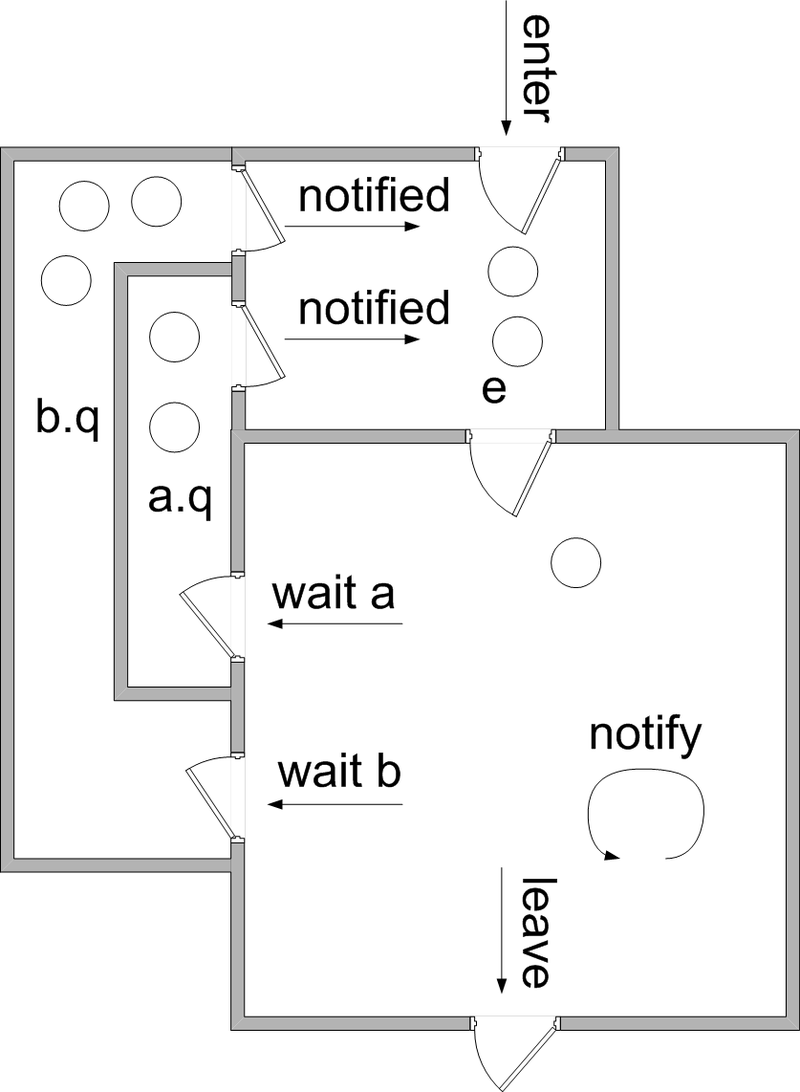
\includegraphics[width=0.35\textwidth]{./pics/CondScheme.png}};
\end{tikzpicture}

One of possible high-level designs:
\begin{itemize}
    \item Mutex: Owner
    \begin{itemize}
        \item The only thread inside critical section        
    \end{itemize}
    \item Mutex: EnterSet
    \begin{itemize}
        \item Threads trying to enter critical section
        \item \textbf{Admission policy for lock acquisition}
    \end{itemize}
    \item Condition: WaitSet
    \begin{itemize}
        \item Threads waiting for signal and now out of critical section
        \item \textbf{Admission policy for notification}
    \end{itemize}    
\end{itemize}
\end{frame}

\questiontime{what is the connection between starvation and admission policy?}
\questiontime{what is the connection between fairness and throughput?}

\begin{frame}[t,fragile]{Fairness and Starvation for Condition Variables}

Short description: fair mutex + unfair \texttt{WaitSet} => unfair system

\begin{minted}{java}
threadA()  { l.lock(); try { while(true) { 
                               System.out.println("A");
                               condition.signal(); condition.await();
}} finally { l.unlock(); }}
threadB()  { l.lock(); try { while(true) {
                               System.out.println("B");
                               condition.signal(); condition.await();
}} finally { l.unlock(); }}
threadC()  { l.lock(); try { while(true) {
                               System.out.println("C");
                               condition.signal(); condition.await();
}} finally { l.unlock(); }}
\end{minted}

\pause
\texttt{A, B, A, B, A, B ...}
\end{frame}

\begin{frame}[t,fragile]{Unbounded concurrent queue}

\begin{itemize}
    \item Thread-safe FIFO container    
\end{itemize}

\begin{minted}{java}
class LockedFIFO<T> implements Queue<T> {
    private final Queue<T> q = new LinkedList<>();
    private final Lock l = new ReentrantLock();
    boolean offer(T e) { l.lock(); try { return q.offer(e); } finally { l.unlock(); }}
    T poll()           { l.lock(); try { return q.poll();   } finally { l.unlock(); }}
    boolean isEmpty()  { l.lock(); try { return q.isEmpty();} finally { l.unlock(); }}
}
\end{minted}
\end{frame}

\questiontime{could you estimate the size of \texttt{LockedFIFO}?}

\begin{frame}[t,fragile]{Bounded concurrent queue}

\begin{itemize}
    \item FIFO container with fixed size
\end{itemize}

\end{frame}

\questiontime{what submitting thread should do when queue is full?}
\questiontime{what executor thread should do when queue is empty?}

\begin{frame}[t,fragile,noframenumbering]{Bounded concurrent queue}

\begin{itemize}
    \item FIFO container with fixed size and blocking methods
\end{itemize}

\pause
\texttt{BlockingQueue<E>}\footnote<2->{\tiny\url{https://docs.oracle.com/en/java/javase/11/docs/api/java.base/java/util/concurrent/BlockingQueue.html}}
\begin{minted}{java}
interface BlockingQueue<E> {
    void put(E e);
    E take();
}
\end{minted}
\pause

Mmmm... \texttt{add}, \texttt{offer}, \texttt{put}, \texttt{remove}, \texttt{poll} ...

\end{frame}

\begin{frame}[t,fragile,noframenumbering]{Bounded concurrent queue}

\begin{itemize}
    \item FIFO container with fixed size and blocking methods
\end{itemize}

\begin{minted}{java}
interface BlockingQueue<E> {
    void put(E e);
    E take();
}
\end{minted}
\pause

\begin{center} Refresher on Java stdlib collections\footnote<2->{\tiny\url{https://docs.oracle.com/en/java/javase/11/docs/api/java.base/java/util/concurrent/BlockingQueue.html}} \end{center}
\newline

\begin{tabular}{l|llll}
         &    Throws exception  &  Special value &  Blocks  & Times out            \\
\hline
Insert   &    add(e)            &  offer(e)      &  put(e)  & offer(e, time, unit) \\
Remove   &    remove()          &  poll()        &  take()  & poll(time, unit)     \\
Examine  &    element()         &  peek()        &  N/A     & N/A                  \\
\end{tabular}

\end{frame}

\begin{frame}[t,fragile]{Bounded concurrent queue with single condition}

\begin{minted}{java}
class BoundedBuffer<E> implements BlockingQueue<E> {
  Lock l = new ReentrantLock(); 
  Condition c = lock.newCondition();
  Queue<E> q = new LinkedList<>();
  ...
\end{minted}

\end{frame}

\begin{frame}[t,fragile,noframenumbering]{Bounded concurrent queue with single condition}

\begin{minted}{java}
class BoundedBuffer<E> implements BlockingQueue<E> { Lock l; Condition c; Queue<E> q;
  ...
\end{minted}

\end{frame}

\begin{frame}[t,fragile,noframenumbering]{Bounded concurrent queue with single condition}

\begin{minted}{java}
class BoundedBuffer<E> implements BlockingQueue<E> { Lock l; Condition c; Queue<E> q;
  void put(E x) { l.lock(); try {
      ???
      ???
    } finally { l.unlock(); }}
  E take() { lock.lock(); try {
      ???
      ???
      ???
    } finally { l.unlock(); }}}
\end{minted}
\end{frame}

\begin{frame}[t,fragile,noframenumbering]{Bounded concurrent queue with single condition}

\begin{minted}{java}
class BoundedBuffer<E> implements BlockingQueue<E> { Lock l; Condition c; Queue<E> q;
  void put(E x) { l.lock(); try {
      while (q.size() == MAX_CAPACITY) { c.await(); }
      q.add(x); c.signal();
    } finally { l.unlock(); }}
  E take() { lock.lock(); try {
      ???
      ???
      ???
    } finally { l.unlock(); }}}
\end{minted}
\end{frame}

\begin{frame}[t,fragile,noframenumbering]{Bounded concurrent queue with single condition}

\begin{minted}{java}
class BoundedBuffer<E> implements BlockingQueue<E> { Lock l; Condition c; Queue<E> q;
  void put(E x) { l.lock(); try {
      while (q.size() == MAX_CAPACITY) { c.await(); }
      q.add(x); c.signal();
    } finally { l.unlock(); }}
  E take() { lock.lock(); try {
      while (q.isEmpty()) { c.await(); }
      c.signal();
      return q.remove();
    } finally { l.unlock(); }}}
\end{minted}
\pause
\textbf{Reminder}: \texttt{signal} wakes up one of waiting threads
\pause
\newline
Assume: \texttt{MAX\_CAPACITY = 2}, \texttt{q.size() == 2}, 3 blocked \texttt{put}s
\pause
\newline
Scenario: 3 \texttt{take}s, last still hangs
\end{frame}

\begin{frame}[t,fragile]{Homework: analysis of bounded concurrent queue with single condition}

{\tiny\url{https://github.com/Svazars/parallel-programming/blob/main/hw/block1/3.4/readme.markdown}}
\begin{homeworkmail}{Task 3.4}
    Prove that for any \texttt{MAX\_CAPACITY > 2} there exists concurrent execution scenario where
    \texttt{take} operation indefinitely blocks despite the fact that queue contains some elements.
\end{homeworkmail}

\end{frame}


\subsection{Multiple condition variables per lock}
\showTOCSub

\begin{frame}[t,fragile]{Bounded concurrent queue with two conditions}

\begin{minted}{java}
class BoundedBuffer<E> implements BlockingQueue<E> { Lock l; Queue<E> q;
  Condition notFull  = l.newCondition(); 
  Condition notEmpty = l.newCondition(); 
  void put(E x) { 
      ???
      ???
      ???}
  E take() {
      ???
      ???
      ???
      ???}
\end{minted}
\end{frame}

\begin{frame}[t,fragile,noframenumbering]{Bounded concurrent queue with two conditions}

\begin{minted}{java}
class BoundedBuffer<E> implements BlockingQueue<E> { Lock l; Queue<E> q;
  Condition notFull  = l.newCondition(); 
  Condition notEmpty = l.newCondition(); 
  void put(E x) { l.lock(); try {
      ???
      ???
    } finally { l.unlock(); }}
  E take() { lock.lock(); try {
      ???
      ???
      ???
    } finally { l.unlock(); }}}
\end{minted}
\end{frame}


\begin{frame}[t,fragile,noframenumbering]{Bounded concurrent queue with two conditions}

\begin{minted}{java}
class BoundedBuffer<E> implements BlockingQueue<E> { Lock l; Queue<E> q;
  Condition notFull  = l.newCondition(); 
  Condition notEmpty = l.newCondition(); 
  void put(E x) { l.lock(); try {
      while (q.size() == MAX_CAPACITY) { notFull.await(); }
      q.add(x); notEmpty.signal();
    } finally { l.unlock(); }}
  E take() { lock.lock(); try {
      while (q.isEmpty()) { notEmpty.await(); }
      notFull.signal();
      return q.remove();
    } finally { l.unlock(); }}}
\end{minted}

\pause Seems OK ... \pause Official javadoc: {\tiny\url{https://docs.oracle.com/en/java/javase/11/docs/api/java.base/java/util/concurrent/locks/Condition.html}}

\end{frame}

\begin{frame}[t,fragile]{Concurrent queues}

\begin{itemize}
    \item Bounded array-based buffer {\tiny\url{https://docs.oracle.com/en/java/javase/11/docs/api/java.base/java/util/concurrent/ArrayBlockingQueue.html}}

    \item Optionally limited-length linked list {\tiny\url{https://docs.oracle.com/en/java/javase/11/docs/api/java.base/java/util/concurrent/LinkedBlockingQueue.html}}

    \item Elements with priorities \newline {\tiny\url{https://docs.oracle.com/en/java/javase/11/docs/api/java.base/java/util/concurrent/PriorityBlockingQueue.html}}
\end{itemize}
\end{frame}

\subsection{Predicate invalidation}
\showTOCSub

\begin{frame}[t,fragile]{Predicate invalidation}

Short description: thread \texttt{await}s for predicate and \textbf{does not recheck} it upon wakeup

\begin{minted}{java}
threadA() { lock.lock(); try {
        while (true) {
            if (data == null) condition.await();
            System.out.println(data.hashCode())            
        }
    } finally { lock.unlock(); } 
}
threadB() { while (true) {
        lock.lock(); try {
            if (random.nextBoolean()) { data = null; } 
            else { data = new Data(); condition.signal(); }
        } finally { lock.unlock(); }
    }
}
\end{minted}
\end{frame}

\begin{frame}[t,fragile,noframenumbering]{Predicate invalidation}

Short description: thread \texttt{await}s for predicate and \textbf{does not recheck} it upon wakeup

Solution: \textbf{always} re-check \texttt{await} predicate. If it is invalidated, wait again. 

\textbf{Ensure} you are not suffering from missing signal bug.
\end{frame}

\begin{frame}{Condition variable}
\framesubtitle{Conclusion}

\begin{itemize}
    \item Cross-thread message passing/coordination \textbf{could} be implemented via mutex + polling    
    \item Signalling saves computation resources for something more useful than busy looping
\end{itemize}

Mutex + ConditionalVariable allow to build custom synchronization protocols. Be aware of
\begin{itemize}
    \item Lost signal problem    
    \item Spurious wakeup
    \item Fairness considerations
    \item Predicate invalidation
\end{itemize}
\end{frame}

\begin{frame}{Homework}

{\tiny\url{https://github.com/Svazars/parallel-programming/blob/main/hw/block1/3.5/readme.markdown}}
\begin{homeworkmail}{Task 3.5}
    Open \url{https://deadlockempire.github.io}, pass ''Condition Variables'' level.
\end{homeworkmail}
\end{frame}

\questiontime{why are we trying to implement every single bit of \texttt{java.util.concurrent}: \texttt{Future}, \texttt{ExcutorService}, \texttt{BlockingQueue}?}

\section{Thread pools}
\showTOC

\begin{frame}[fragile]{ExecutorService: real world API}

ExecutorService\footnote{\tiny\url{https://docs.oracle.com/en/java/javase/11/docs/api/java.base/java/util/concurrent/ExecutorService.html}}

\begin{minted}{java}
  void execute(Runnable command) // implements Executor
  <T> Future<T> submit(Callable<T> task)   
  <T> T invokeAny(Collection<Callable<T>> tasks) // returns any successful
  void shutdown() // no new tasks
  List<Runnable> shutdownNow() // try stop all executing, return all pending
  boolean awaitTermination(long timeout, TimeUnit unit)
\end{minted}

Structured concurrency:
\begin{itemize}
    \item Asynchronous result (\texttt{Future})
    \item Conditional execution (\texttt{invokeAny})
    \item Life cycle management (\texttt{submit}, \texttt{shutdown}, \texttt{awaitTermination})
\end{itemize}

\end{frame}

%\questiontime{What if somebody \texttt{submit} task with unhandled exception to \texttt{ExecutorService}? What about other ways to ''destroy'' thread?}

\begin{frame}[fragile]{ScheduledExecutorService}

ScheduledExecutorService\footnote{\tiny\url{https://docs.oracle.com/en/java/javase/11/docs/api/java.base/java/util/concurrent/ScheduledExecutorService.html}}

\begin{minted}{java}
// Value-returning one-shot task that becomes enabled after the given delay
<V> ScheduledFuture<V> schedule(Callable<V> callable, long delay, 
                                TimeUnit unit);
// Periodic action that becomes enabled first after the given initial delay 
// Executions will start after `initialDelay`, then `initialDelay + period` ...
ScheduledFuture<?>  scheduleAtFixedRate(Runnable command, long initialDelay, 
                                        long period, TimeUnit unit);
\end{minted}

Delay and periodic schedule control.

\textbf{Hint}: could be useful for testing, stress measurements and simulating ''workload bursts''.
\end{frame}


\begin{frame}[fragile]{ThreadPools API: summary}

\begin{itemize}
    \item \texttt{Runnable}, \texttt{Callable<T>} -- unit of work (e.g. tasks)
    \item \texttt{ThreadFactory} -- environment requirements (e.g. threads)
    \item \texttt{Executor} -- submission point (e.g. thread-safe container)
    \item \texttt{ExecutorService} -- task execution policy (life cycle, resource limits, frequency)
\end{itemize}

\pause

\textbf{Bad news}: you do not know which thread will execute your code.
\begin{itemize}
    \item blocking methods, unexpected lock order, deadlocks, race conditions, data races
\end{itemize}

\pause

\textbf{Good news}: you do not know which thread will execute your code.
\begin{itemize}
    \item under-the-hood synchronization ''just works'', nothing to implement
\end{itemize}
\end{frame}

\questiontime{no deadlock when all submitted tasks have no \texttt{Lock}s and \texttt{Condition}s inside?}

\begin{frame}[t,fragile]{ThreadPools API pitfalls: thread-starvation deadlock}

\begin{minted}{java}
var service = new SingleThreadExecutorService();
var outerFuture = service.submit(() -> {
    var innerFuture1 = service.submit(() -> {
        return compute(1);
    });
    var innerFuture2 = service.submit(() -> {
        return compute(2);
    });
    return innerFuture1.get() + innerFuture2.get();
});
\end{minted}

\pause
Single working thread waits for future to be computed by himself.
\end{frame}

\begin{frame}[t,fragile]{ThreadPools API pitfalls: resource deadlock}

\begin{minted}{java}
var service = new FixedThreadPool(2);
var result = service.submit(() -> {
               return service.submit(() -> {
                 return service.submit(() -> {
                    return compute(1);
                 }).get();
               }).get();;
             }).get();
\end{minted}

\newline
\pause \texttt{Future.get} that does not block but helps with pending tasks? 
\newline
\pause \texttt{CompletableFuture}, \texttt{ForkJoinTask} ... \pause Not today.

\end{frame}

\questiontime{is it always a good idea to use \texttt{ExecutorService} that creates threads on demand?}

\begin{frame}[t,fragile]{ThreadPools API pitfalls: denial of service}

\begin{minted}{java}
var service = new ThreadPerTaskExecutorService();
for (Data request: userRequests) {
    service.submit(() -> {
        return process(request);
    });
}
\end{minted}

\pause
Too many requests could cause \texttt{OutOfMemory: too much threads}.

\end{frame}

\begin{frame}[fragile]{ThreadPools API: available implementations}

Executors\footnote{\tiny\url{https://docs.oracle.com/en/java/javase/11/docs/api/java.base/java/util/concurrent/Executors.html}}

\begin{minted}{java}
static ExecutorService newFixedThreadPool(int nThreads, ThreadFactory tFactory);
static ExecutorService newSingleThreadExecutor(ThreadFactory threadFactory);
static ExecutorService newCachedThreadPool(ThreadFactory threadFactory);
\end{minted}

\pause

Remember:
\begin{itemize}
    \item Fixed-size thread pools may cause resource deadlock
    \item Single-thread executor not necessarily use the same thread
    \item Caching can cause memory leaks or unintentionally reuse resources (e.g. native-lib-specific resources)
\end{itemize}

Full overview and arbitrary customization available\footnote<2->{\tiny\url{https://docs.oracle.com/en/java/javase/11/docs/api/java.base/java/util/concurrent/ThreadPoolExecutor.html}}

\end{frame}

% \begin{frame}[fragile]{ThreadPools API: homework}
% 
% TODO task 3.6.1
% implement newFixedThreadPool
% reminder: Exception from Callable -- possible Future result
%           any other Throwable -- thread should die (abnormal situation), future still returns exception
%           died threads should be restored by executor mechanics (factory)
% 
% TODO task 3.6.2
% implement newCachedThreadPool
% reminder: unused threads should be killed (e.g. after 10 seconds)
% 
% TODO task 3.6.3
% implement selfHelpingThreadPool
% N workers
% when thread invokes blocking Future.get and it is not still ready -- this thread executes task
% 
% caveats: extra grabbed locks in helper
%          properly delete task from queue
% 
% \end{frame}

\begin{frame}[fragile]{ThreadPools API: now you know it}

From now on, you \textbf{must} avoid using \texttt{new Thread()} in your solutions.

\begin{itemize}
    \item Use existing \texttt{ExecutorService}s
    \item Create custom \texttt{ThreadPoolExecutor}s
    \item Encapsulate thread configuration in \texttt{ThreadFactory}
\end{itemize}

\end{frame}

\section{Summary}

\begin{frame}{Summary}
\begin{itemize}
    \item Decoupling tasks -- \texttt{Runnable}, \texttt{Callable}
        \begin{itemize}
            \item from particular threads  -- \texttt{ThreadFactory}
            \item from submission protocol -- \texttt{Executor}
            \item from scheduling policy   -- \texttt{ExecutorService}
        \end{itemize}
    \item Backoff policies for polling -- better CPU utilization by sacrificing latency
        \begin{itemize}
            \item NoBackoff, FixedBackoff, ExponentialBackoff
        \end{itemize}
    \item Condition variable allows to replace polling with OS-level signalling
        \begin{itemize}
            \item lost signal, spurious wakeups, fairness, predicate invalidation
        \end{itemize}
    \item Every thread pool type has
        \begin{itemize}
            \item advantages: life cycle management, delayed execution, on-demand thread creation
            \item weaknesses: thread-starvation deadlock, resource deadlock, denial of service
        \end{itemize}
\end{itemize}
\end{frame}

\begin{frame}{Summary: homework}

\texttt{Lecture 3, Tasks 3.*:} {\tiny\url{https://github.com/Svazars/parallel-programming/blob/main/hw/block1}}

\end{frame}

% TODO: CompletionService (auto order finished futures, Future.done)


%Big homework (4w)
    %bounded thread pool, blocking awaits are self-helping,
%- design
%- tests
%- deadlock conditions
%- example of deadlock with resource-constrained cause


% \begin{frame}{Producer consumer}
% Unbounded queue with mutex
% \end{frame}
% 
% \begin{frame}{Publisher-subsrciber}
% Pull/push approaches, reactive systems
% \end{frame}
% 
% \begin{frame}{Backoff policies}
% Livelock
% \end{frame}
% 
% \begin{frame}{Problems}
% 
% message passing + backpressure 
% self impl thread-safe counter
% self impl striped lock (hashmap?)
% \end{frame}

\end{document}
